\documentclass[a4paper]{article}
\usepackage[english]{babel}
\usepackage{booktabs}
\usepackage{graphicx}
\usepackage[hidelinks]{hyperref}

\author{Christian Brock\footnote{Dresden Gönnsdorf Observatory}}
\title{Introduction in the scientific method using the Hertzsprung-Russel-Diagram}
\date{July 2025}

\setlength{\parindent}{0pt}
\setlength{\parskip}{1em}

\begin{document}
	\maketitle

    \begin{abstract}
        Use the Hertzsprung-Russel-Diagram (HRD) to introduce the scientific method to students.

        \bigskip
        \center{\textbf{Zusammenfassung}}
        \bigskip

        Der Hertzsprung-Russel-Diagramm (HRD) wird verwendet, um Schülern die wissenschaftlichen Methode näher zu bringen.
    \end{abstract}

   	\section{Introduction}

	In our observatory we tried to introduce the scientific method to a group of students aged 11--13.
    Being an astronomical observatory, we decided to use the Hertzsprung-Russel-Diagram (HRD).

    \section{Lesson structure}

    \subsection*{What is science?}

    Ask the students what science is \footnote{This is easier in German as science translates to Wissenschaft which literally means knowledge creation.}.
    Lead them to the understanding that sciences uses the following method
    \footnote{Most still do and almost all did so in the past}:
    \begin{enumerate}
        \item Observe, Measure, Record
        \item Classify, Analyze, Interpret
        \item Hypothesize, Test, Verify
    \end{enumerate}

    \subsection*{Observe, i.e.\ the stars}

    You can use the night sky, a star globe, some planetarium software such as \url{stellarium.org} or a photo of the night sky.
    
    Goal is to realize that stars have different brightness and color.

    Start to ask questions about the observation, e.g.:
	\begin{itemize}
		\item Do we have stars of all colors?
		\item Do we have stars of all brightnesses?
	\end{itemize}

    \subsection*{Measure}
    
	Before continuing to the next step we need to link color with temperature.
    Most kids are familiar with the blue and yellow part of the candle flames.
    
    With older students you can mention absolute vs.\ apparent magnitude (see section \ref{sec:faq}).

    \subsection*{Classify}

    \paragraph*{Introducing the Hertzsprung-Russel-Diagram}

    Explain that Hertzsprung and Russel had the same questions we asked in the observation section above.
    They found a way to visualize the stars in a diagram.

    Show the empty Hertzsprung-Russel-Diagram (HRD) in figure \ref{fig:hrd-vorlage}.

    Ask the students what's odd about it.
    Explain the axes:
    \begin{itemize}
        \item Brighter stars have lower magnitudes because the Greak astronomer Hipparchus used a scale from 1 to 6,
            where 1 is the brightest and 6 the dimmest.
        \item Temperature goes from hot to cold because 100 years ago, astronomers thought that starts are born hot
            and cool down. This is not true, but the convention is still used.
    \end{itemize}

    \paragraph*{Filling the Hertzsprung-Russel-Diagram}

    Now we want to fill the HRD with stars.
    We use the stars from table \ref{tab:star_table} and the empty diagram from figure \ref{fig:hrd-vorlage}.
    Make sure each students gets a copy of each.
    
    We found that it helps when the teacher joins the students in this task.
    It will make her humble as the task is hard and the students will feel more comfortable.

    \subsection*{Analyzing}

    After filling the HRD, we can analyze it.
    Ask the students to find patterns in the HRD.
    They will find that stars are not randomly distributed, there are different groups of stars.
    
    Note: The stars were ordered randomly. This ensures that also with only 50\% of the star the students should already see some structure.
    
    \subsection*{Interpret}

    Explain the groups and link them to the life cycle of stars.
    Stress that this was discovered much later but that the HRD was an impoortant step in this discovery.

    \section{FAQ}
    \label{sec:faq}

    \begin{description}
        \item[Visual brightness or magnitude]
            All brighness in this document refers to the visual brightness of stars.
            This differs especially for hot stars which are very bright in the ultra violet.
        \item[Absolute brightness or magnitude]
            In this document, we use the absolute brightness of stars.
            The absolute brightness of a star is the brightness it would have at a distance of 10 parsec.
            You may show that the sun is not a very bright star.
    \end{description}

	\section{Material}
	
	\begin{table}[htbp]
    \include{star_table.tex}
	\caption{List of example stars}
	\label{tab:star_table}
	\end{table}

    \begin{figure}[htbp]
        \centering
        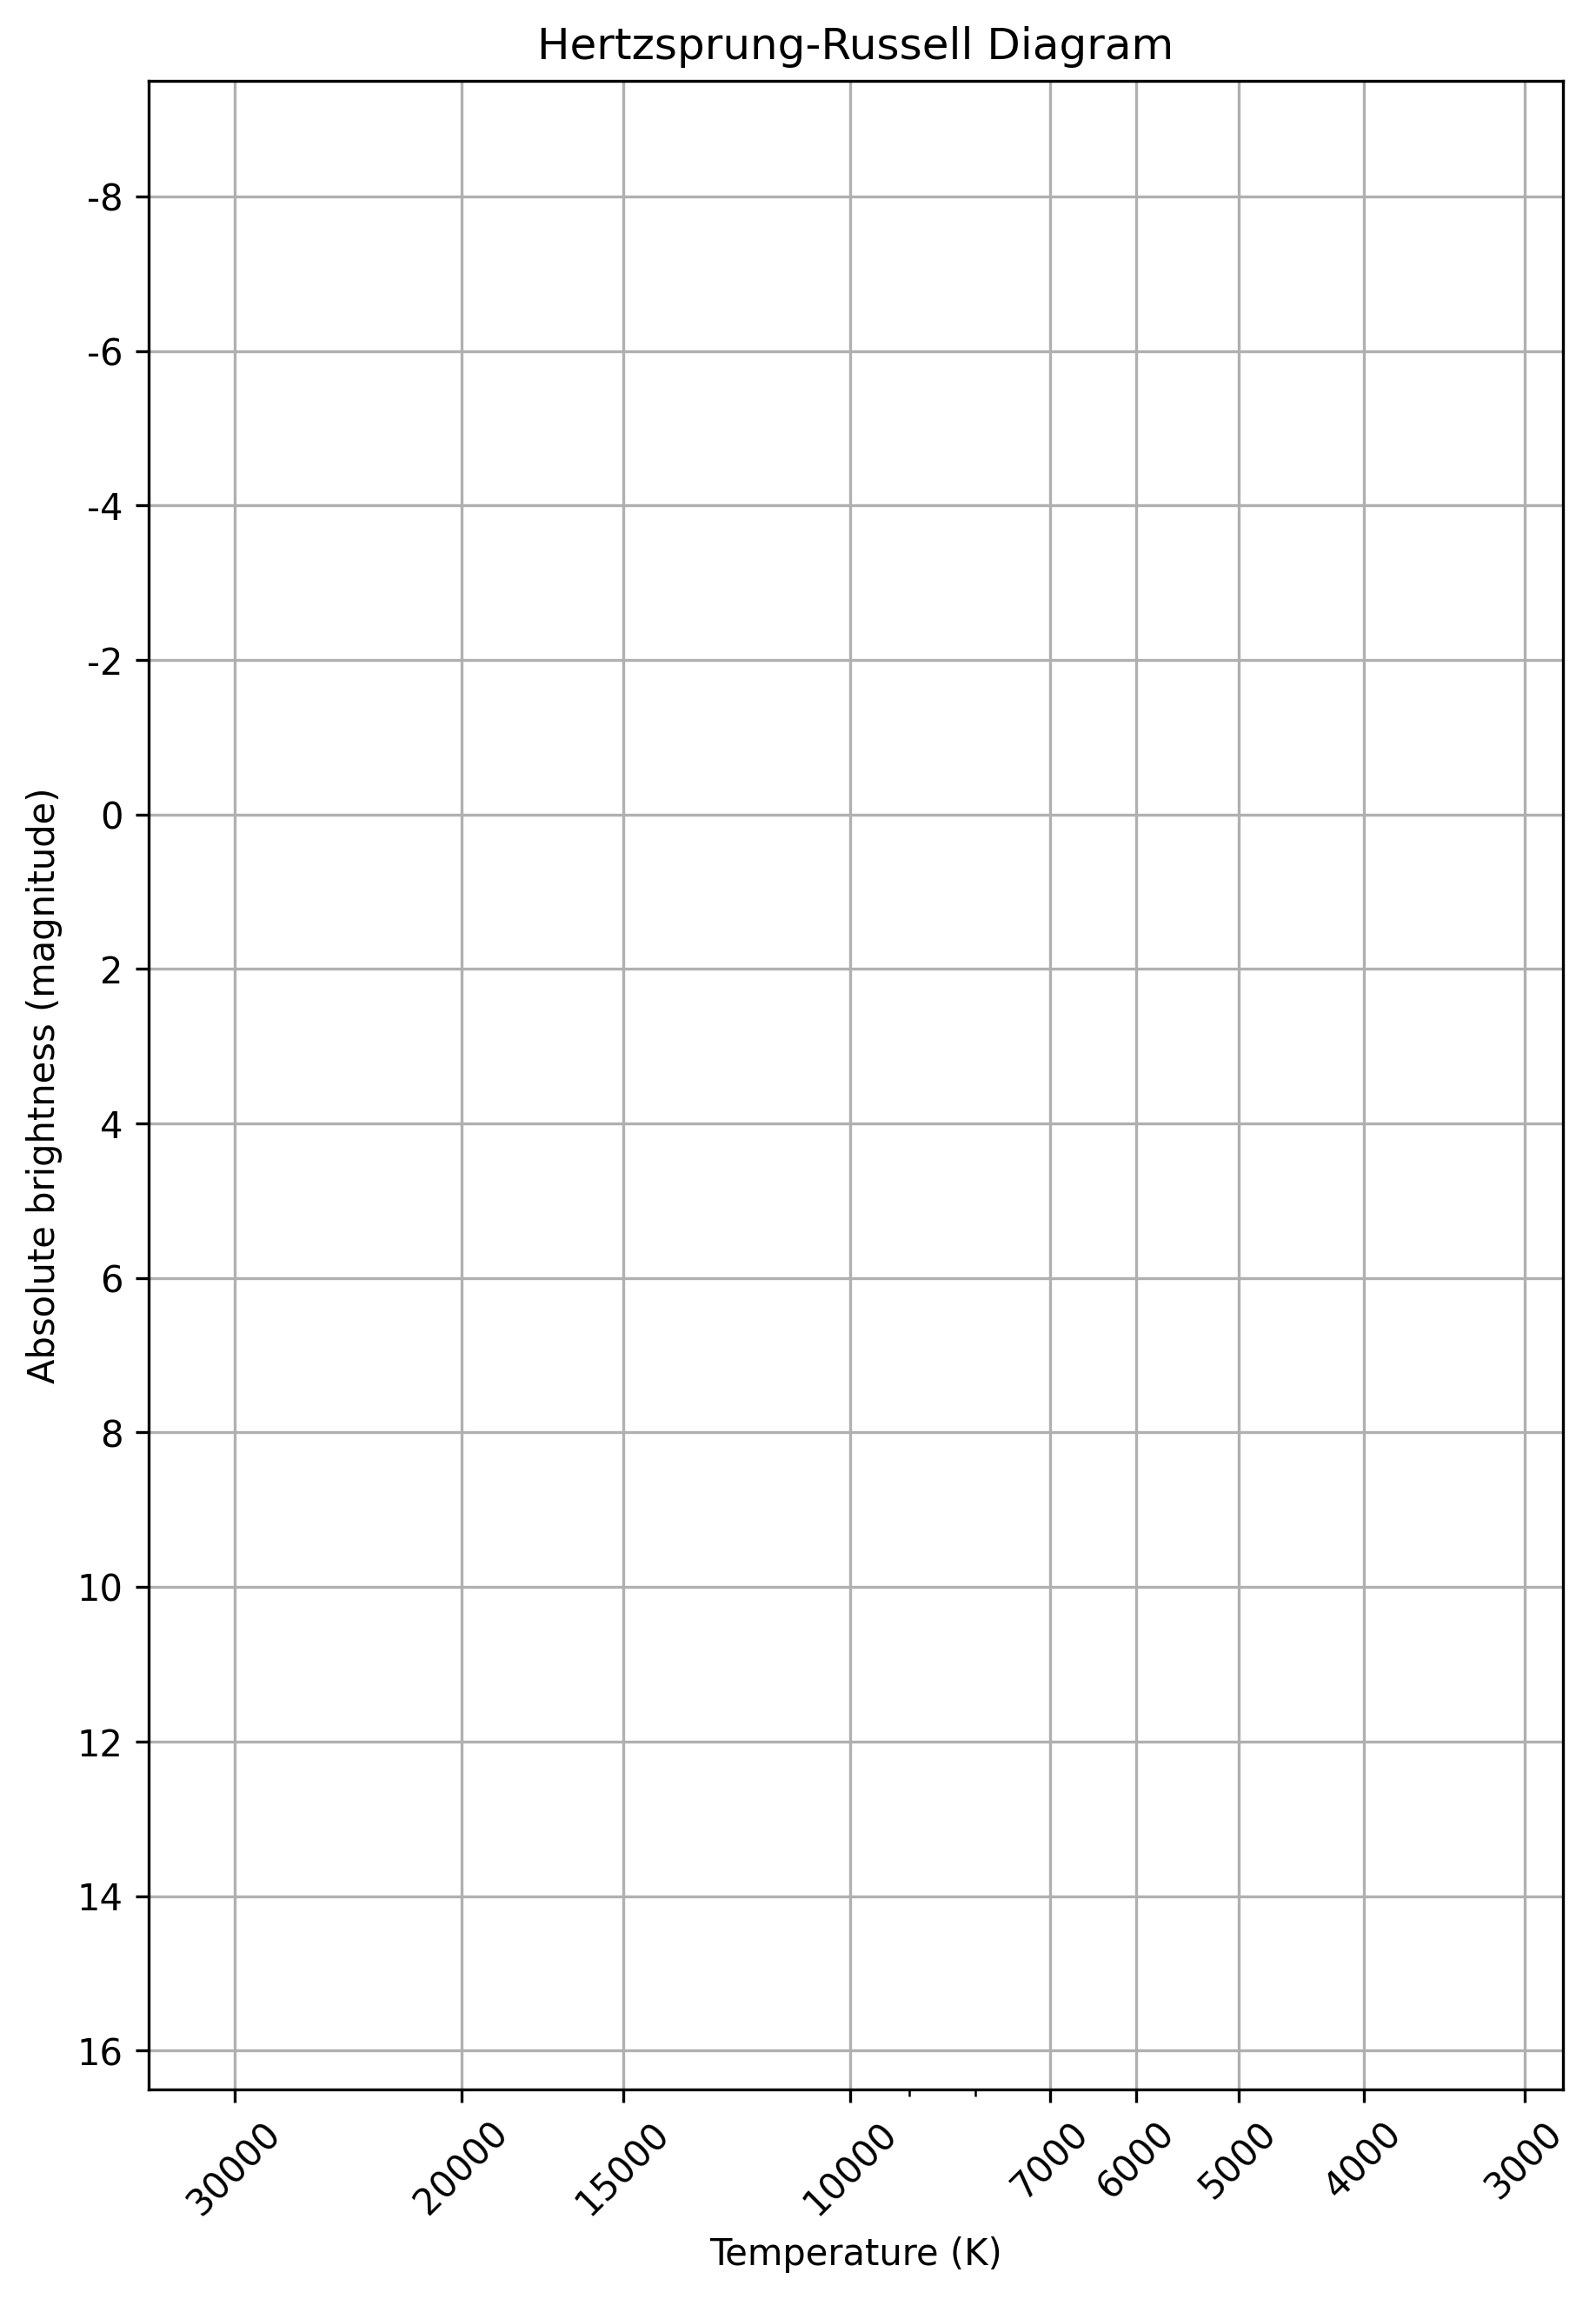
\includegraphics[width=0.8\textwidth]{hrd_empty.png}
        \caption{An empty Hertzsprung-Russel-Diagram (hrd\_empty.png)}
        \label{fig:hrd-vorlage}
    \end{figure}

    \begin{figure}[htbp]
        \centering
        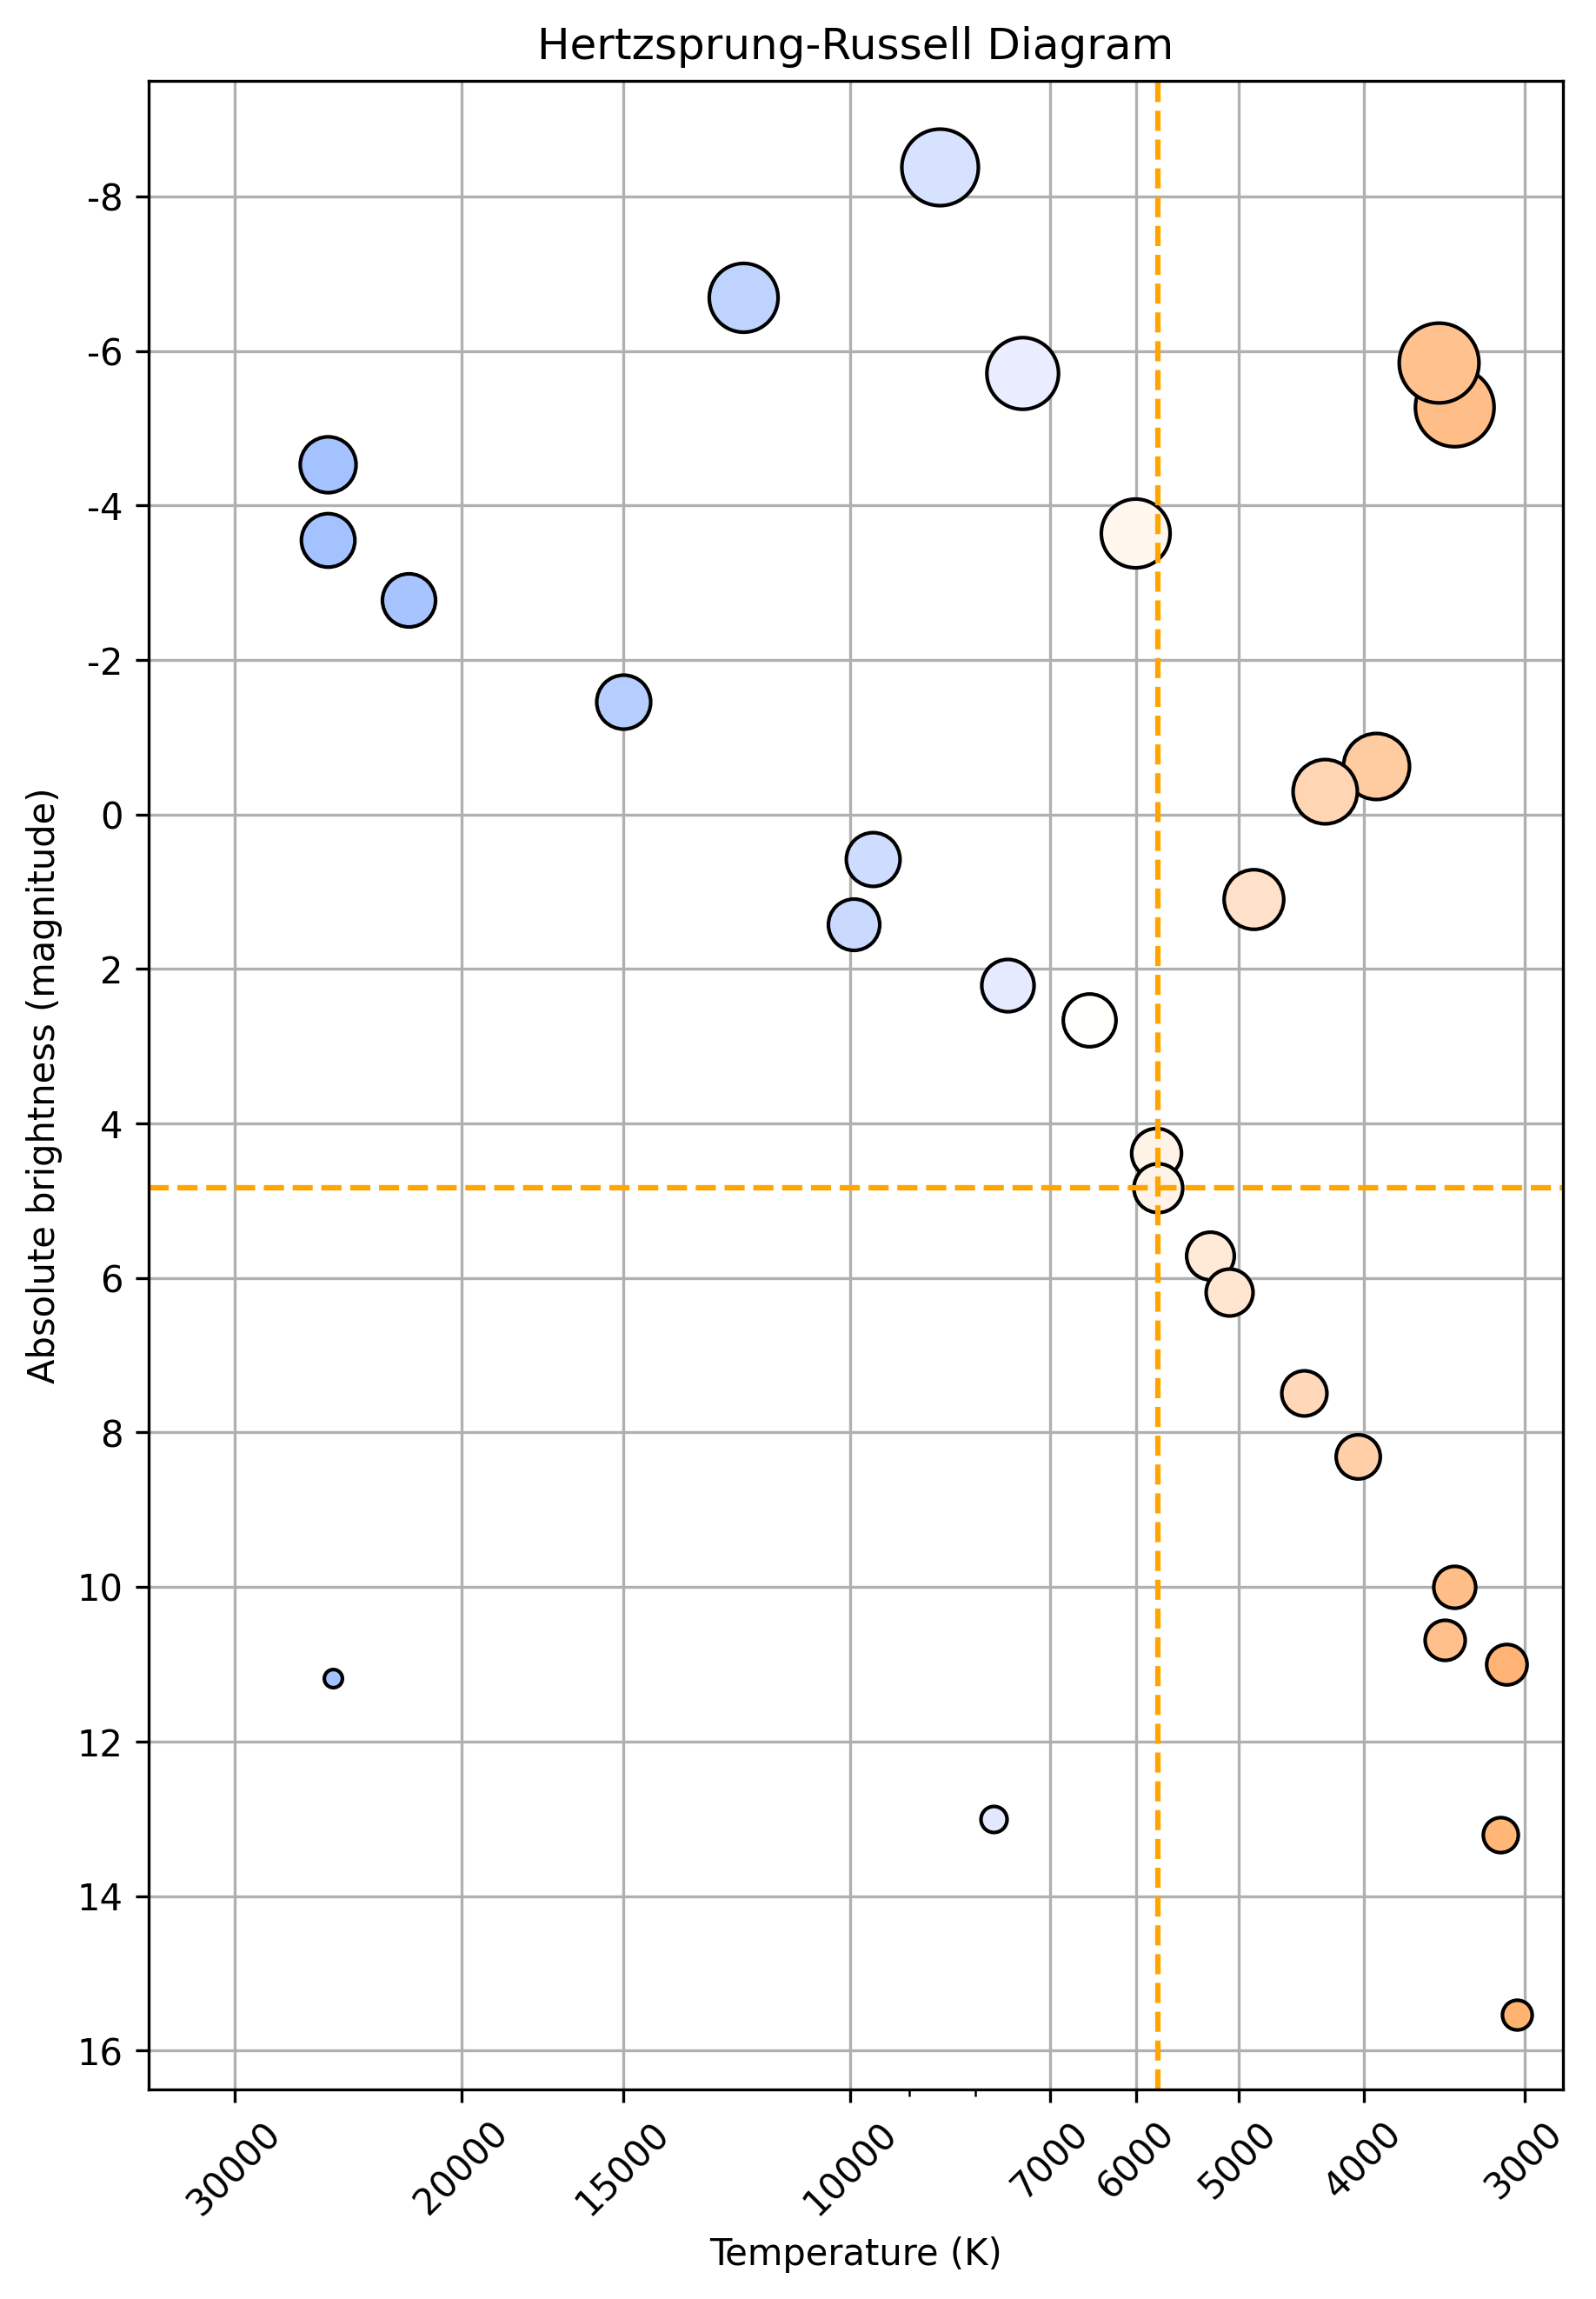
\includegraphics[width=0.8\textwidth]{hrd_with_stars.png}
        \caption{The diagram from figure\ \ref{fig:hrd-vorlage} with stars from table \ref{tab:star_table}.
        	Our home star is marked with dotted lines.}
        \label{fig:hrd-voll}
    \end{figure}

\end{document}
